{\fontsize{12pt}{22pt} \textbf{Local Outlier Factor}\par}

\vspace{5mm}

Local Outlier Factor is an unsupervised method used in anomaly detection. It consists of comparing local density of train observations VS local density of test observations. \\

\underline{Reachability distance} \\

$reachability \mbox{-} distance_k(A,B) = max \{ k \mbox{-} distance (B), d(A,B)\}$  = reachability of A \textit{from} B. \\

$k \mbox{-} distance (B)$: distance from B to its kth nearest neighbor.

The reachability distance of A from B is \textit{at least} the distance between A and B or \textit{at least} the distance of B's neighbor.

When A is very far from B, it's simply the distance between the two points.

When A is very close to B, it's the distance between B and its neighbor. \\

The distance can be computed using different metrics: Euclidean distance, Mahalanobis distance, etc. \\

\underline{Local reachability density} \\

$lrd_k (A) = \frac{1}{\Sigma_{B \in N_k(A)} reachability \mbox{-} distance_k(A,B) / |N_k(A)|}$ \\

It's the inverse of the average of reachability-distances of A from B.

When A is very far from its neighbors: sum of reachability distances is high => local reachability density is small. \\

\underline{Local Outlier Factor} \\

LOF computation consists of comparing the local densities of a point VS its neighbors. \\

$LOF_k(A) : =  \frac{\frac{\Sigma_{B \in N_k(A)}lrd_k(B)}{lrd_k(A)}}{|N_k(A)|}$ \\

$LOF_k(A) > 1$: A is an outlier. Local reachability density of A is small compared to its neighbors.

$LOF_k(A) < 1$: A is an inlier.

\begin{center}
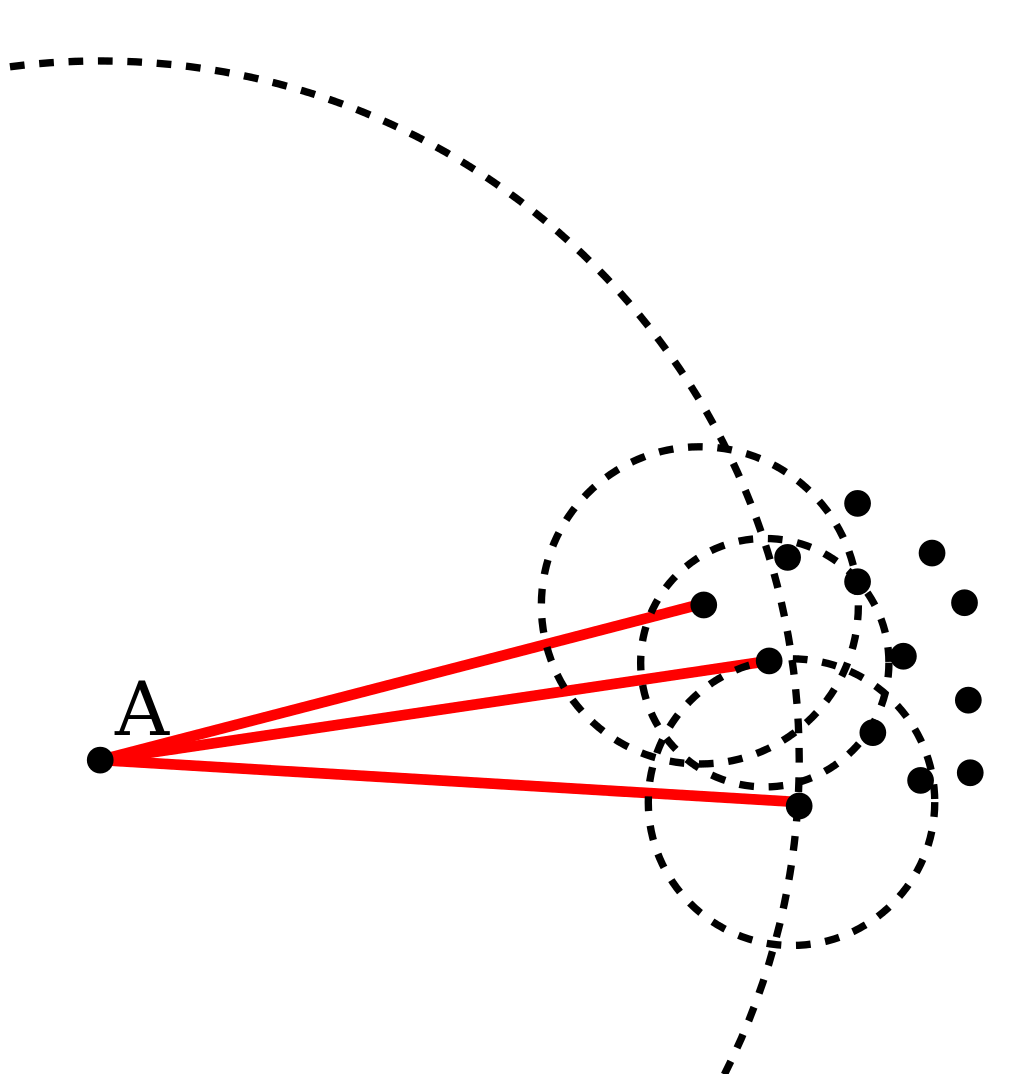
\includegraphics[scale=0.10]{LOF.png}
\end{center}

On this figure, $k = 3$. We can see that the reachability distance of A from its neighbors is high (red segments). The local reachability density of A will thus be \textbf{low}.

On the contrary, the local reachability densities of its neighors is \textbf{high} because each neighbor can be easily reached from their own neighbors.

As a result, LOF would be high so A is an outlier. \\

\underline{sklearn algorithm} \\

To score an observation, \textit{fit} simply memorizes the train observations (same as in knn). 

\textit{score\_samples} first finds the k-nearest neighbors from the train set thanks to the given distance metric. It then computes the local outlier factor for each test observation comparing the test observation local density with its closest k-neighbors local densities in the train set.

\vspace{5mm}